\documentclass{beamer}
\usetheme{metropolis}
\usepackage{graphicx}
\usepackage{subfig}
\usepackage{tcolorbox}
\title{Computer Logic and Digital Circuit Design (PHYS306/COSC330): Unit 1.2}
\author{Jordan Hanson}
\institute{Whittier College Department of Physics and Astronomy}

\begin{document}
\maketitle

\section{Summary}

\begin{frame}{Unit 1.2 Summary - Build a radio from a pile of parts...go!}
\begin{enumerate}
\item Introduction to \textit{mixing} or \alert{heterodyning}
\begin{itemize}
\item The \textbf{transistor} plays a dual role
\item \textbf{Transistors} $\rightarrow$ forthcoming units on logic gates
\end{itemize}
\item The superheterodyne (superhet) radio receiver
\item Through-hole soldering 101
\item The DVM (digital voltmeter)
\item \textbf{Build.} $\rightarrow$ Bonus point for the first team
\end{enumerate}
\end{frame}

\section{Introduction to mixing or heterodyning}

\begin{frame}{Introduction to mixing or heterodyning}
\small
This is not yet \textit{digital} circuit design.  However, the \textbf{AM transistor radio} design was massively popular, taking advantage of new technology: \textbf{transistors}.  Two goals are fulfilled by placing transistors in the design: mixing and amplification.
\begin{figure}
\centering
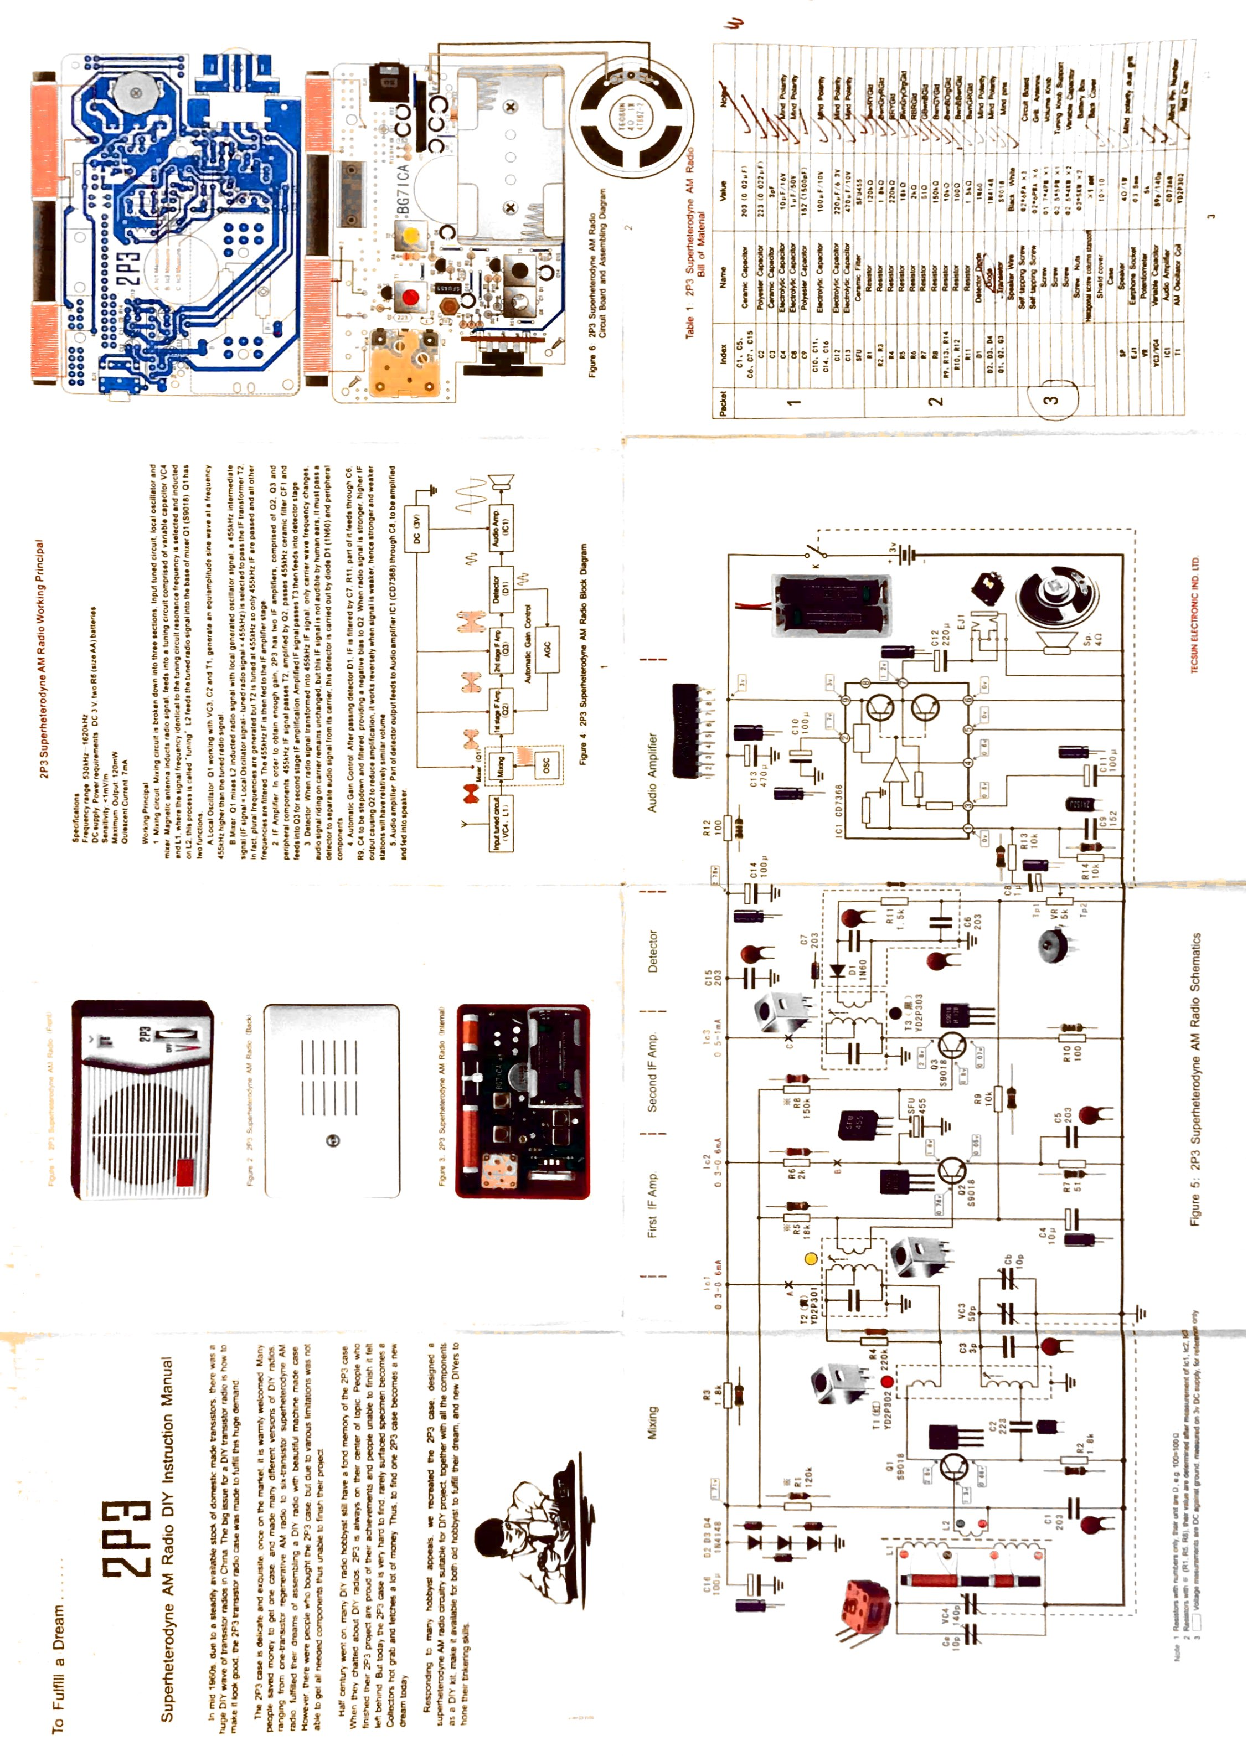
\includegraphics[width=0.4\textwidth,angle=270,trim=6.75cm 15cm 10.5cm 8cm,clip=true]{figures/2P3.pdf}
\end{figure}
\end{frame}

\begin{frame}{Introduction to mixing or heterodyning}
\small
\begin{itemize}
\item AM radio - \textit{amplitude modulation:} the signal data is encoded in amplitude fluctuations.
\item Mixing - the concept of \textit{beat frequencies}
\item Requires stable \alert{local oscillators} at fixed frequency
\end{itemize}
\begin{figure}
\centering
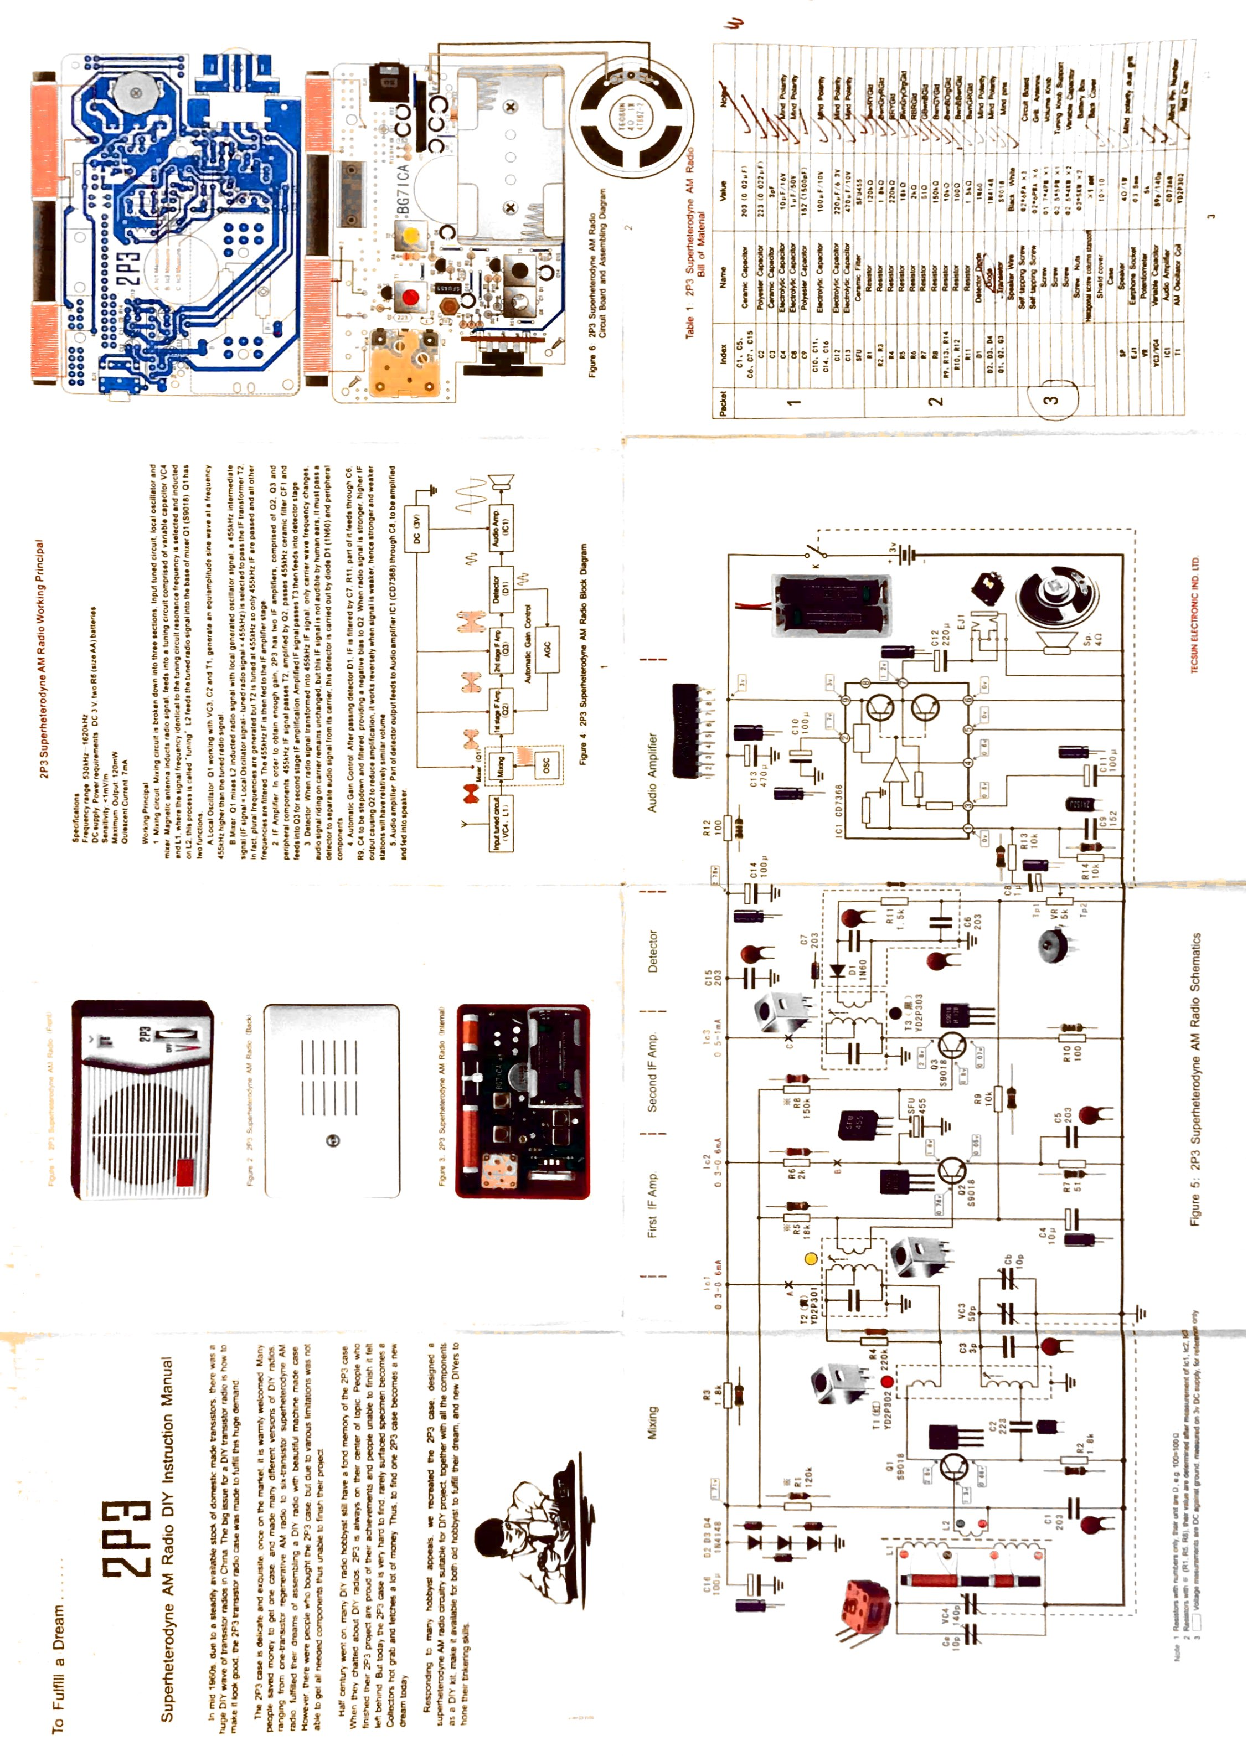
\includegraphics[width=0.4\textwidth,angle=270,trim=6.75cm 15cm 10.5cm 8cm,clip=true]{figures/2P3.pdf}
\end{figure}
\end{frame}

\begin{frame}{Introduction to mixing or heterodyning}
\small
\begin{itemize}
\item Beat frequencies (heterodynes) occur at $f_{r} + f_{lo}$ and $f_{r} - f_{lo}$
\item \textbf{Heterodyning} - make a signal oscillate at $f_{r} + f_{IF}$, then mix with $f_{IF}$ and filter out the higher heterodyne
\item The result: AM radio at $f_{IF}$, with modulations in tact
\item The \textbf{detector} (diodes) grabs only the modulations
\end{itemize}
\begin{figure}
\centering
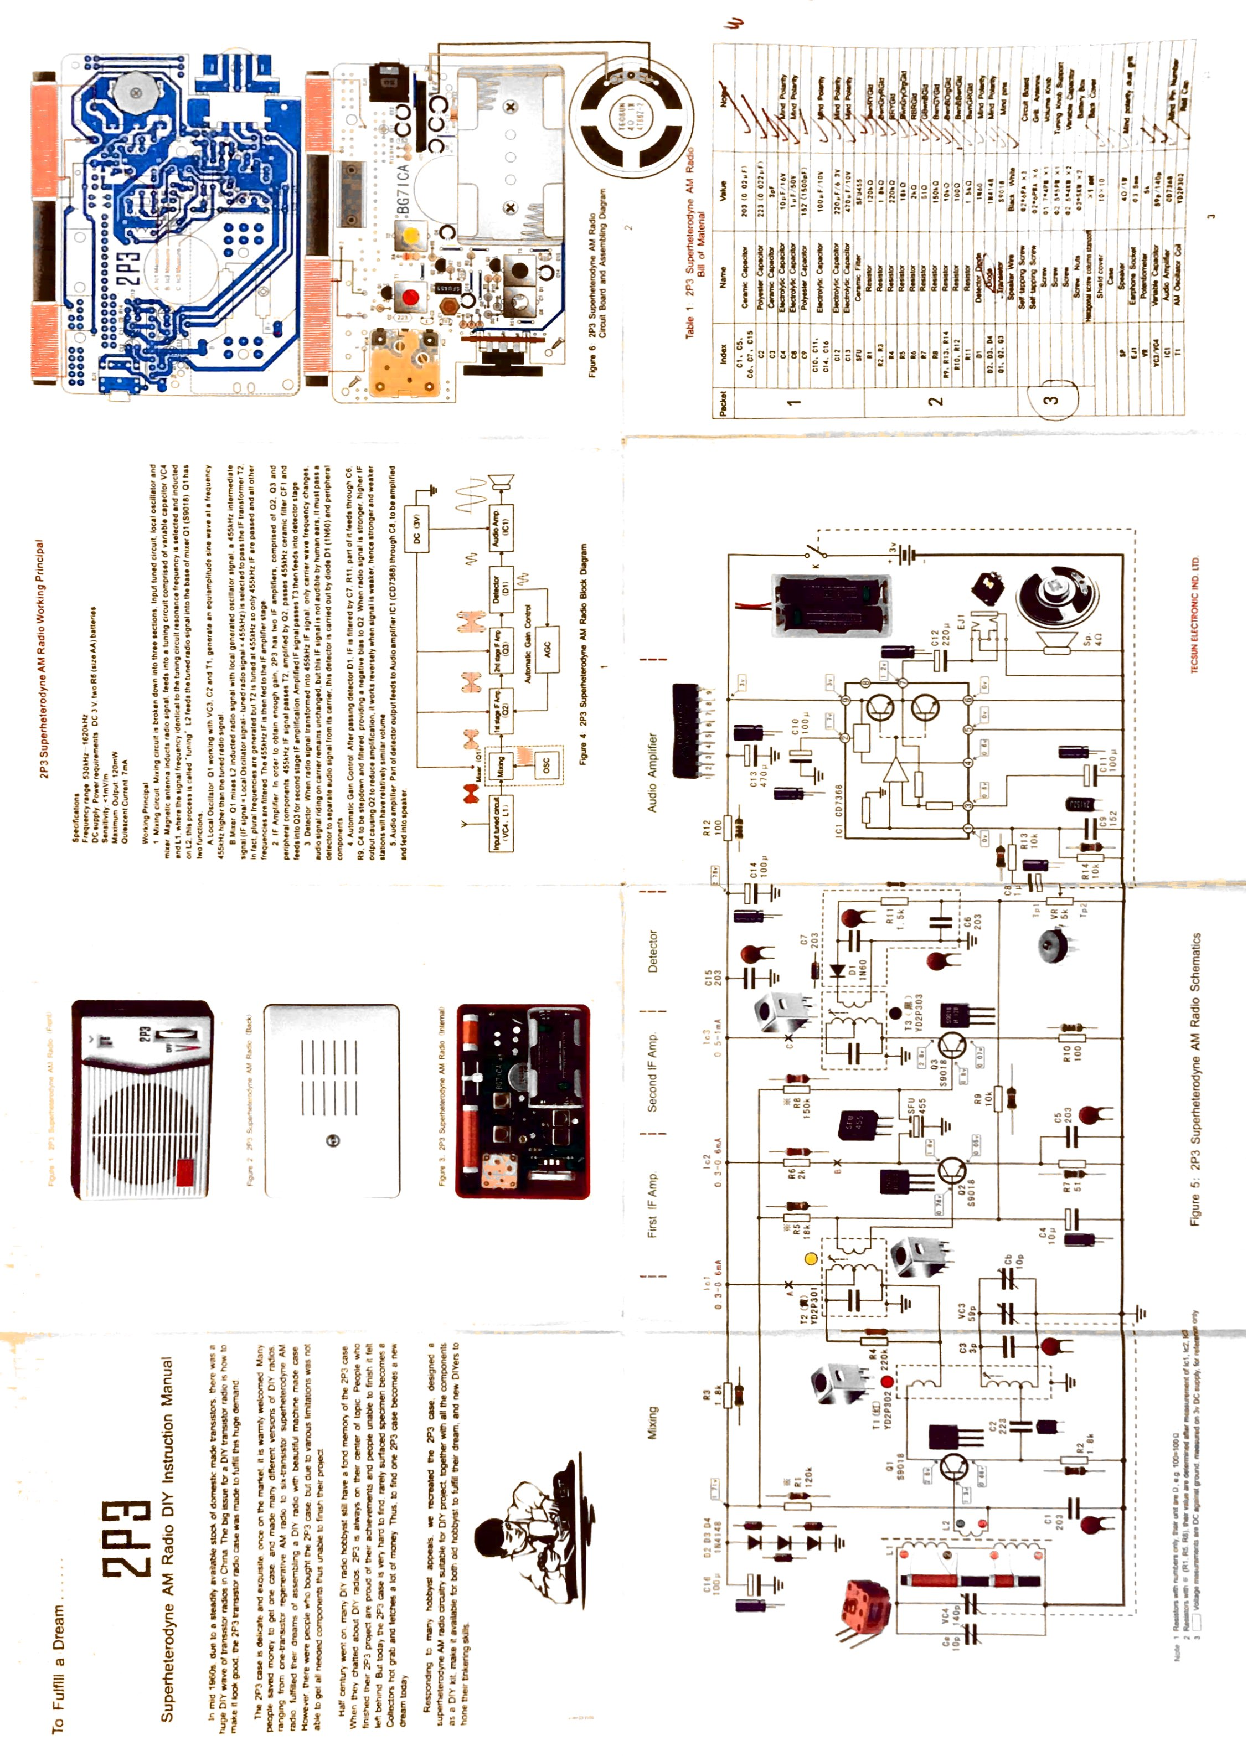
\includegraphics[width=0.4\textwidth,angle=270,trim=6.75cm 15cm 10.5cm 8cm,clip=true]{figures/2P3.pdf}
\end{figure}
\end{frame}

\begin{frame}{Introduction to mixing or heterodyning}
\begin{figure}
\centering
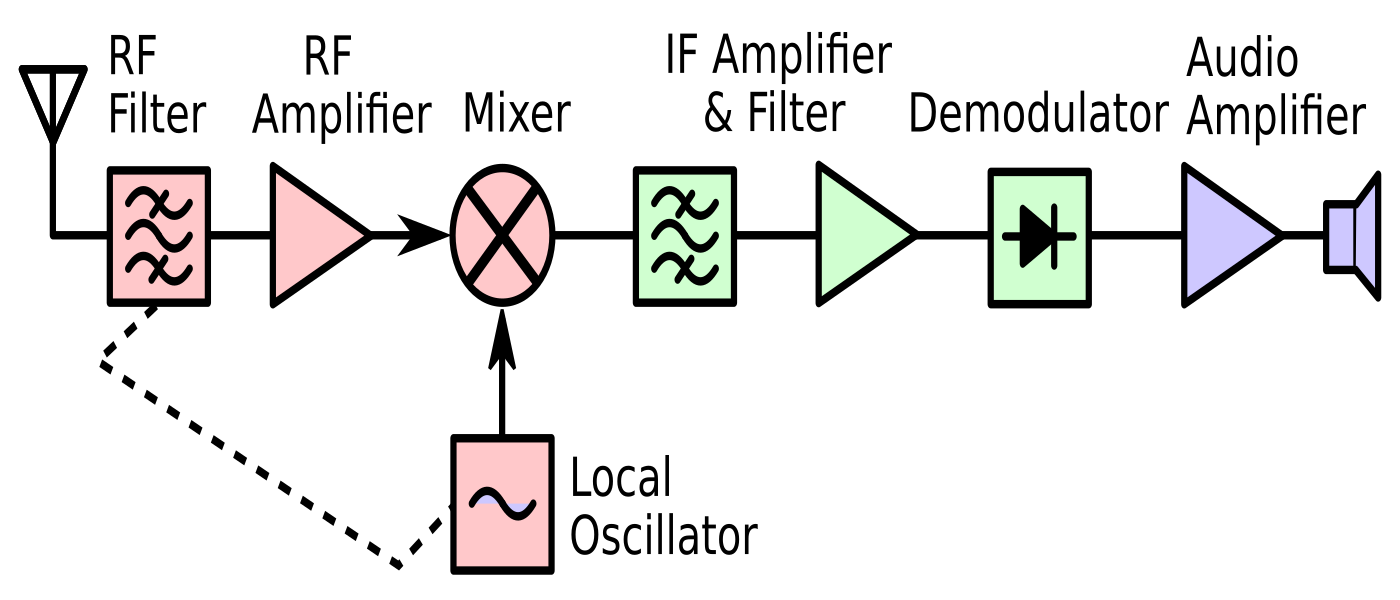
\includegraphics[width=\textwidth]{figures/superhetWiki.png}
\caption{\label{fig:superHet} Source: Wikipedia.  A superheterodyne AM receiver uses an intermediate frequency (IF) to capture the audio modulations.}
\end{figure}
\end{frame}

\section{Introduction to transistors}

\begin{frame}{Introduction to transistors}
\begin{itemize}
\item How does a mixer use the transistor?
\item How does a transistor work?
\item We will use this as an opportunity to learn how transistors may be used to form digital circuits.
\end{itemize}
\begin{figure}
\centering
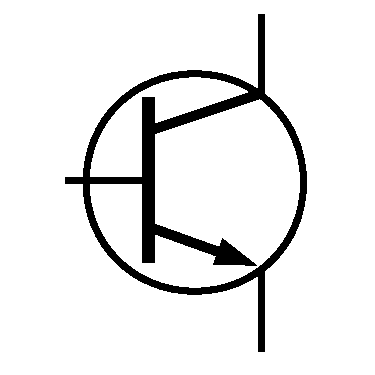
\includegraphics[width=0.25\textwidth]{figures/transistor.pdf}
\caption{\label{fig:transistor} The schematic symbol for the transistor, including the \textit{emitter}, \textit{base}, and \textit{collector}. Amplified (positive) current flows from the emitter to the collected when the base has a positive voltage.}
\end{figure}
\end{frame}

\begin{frame}{Introduction to transistors}
\begin{itemize}
\item \alert{How does a mixer use the transistor?}
\item How does a transistor work?
\item We will use this as an opportunity to learn how transistors may be used to form digital circuits.
\end{itemize}
\begin{figure}
\centering
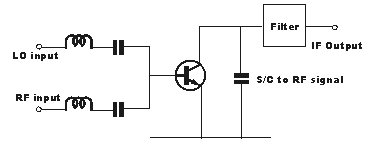
\includegraphics[width=0.6\textwidth]{figures/BJT.png}
\caption{\label{fig:bjt} The bipolar-junction transistor mixer.  A local oscillator is connected in parallel with the \textit{base} of the bipolar transistor.  Positive current flows from the emitter to the collector when \textit{either} the oscillator oscillates or the radio antenna oscillates.  The capacitor at right soaks up unwanted high frequencies.}
\end{figure}
\end{frame}

\begin{frame}{Introduction to transistors}
\begin{itemize}
\item \alert{How does a mixer use the transistor?}
\item How does a transistor work?
\item We will use this as an opportunity to learn how transistors may be used to form digital circuits.
\end{itemize}
\begin{figure}
\centering
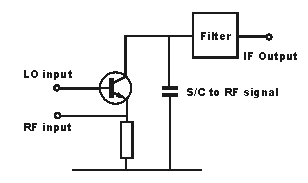
\includegraphics[width=0.4\textwidth]{figures/BJT2.png}
\caption{\label{fig:bjt2} The bipolar-junction transistor mixer.  In this example the radio frequency (RF) input is connected to the emitter and the LO is connected to the base.  One more level of complexity and we have a circuit close to that of the 2P3...}
\end{figure}
\end{frame}

\begin{frame}{Introduction to transistors}
\begin{itemize}
\item \alert{How does a mixer use the transistor?}
\item How does a transistor work?
\item We will use this as an opportunity to learn how transistors may be used to form digital circuits.
\end{itemize}
\begin{figure}
\centering
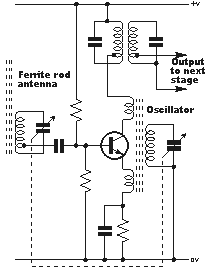
\includegraphics[width=0.25\textwidth]{figures/BJT3.png}
\caption{\label{fig:bjt3} In this final example, the LO and the mixer are combined into one circuit.}
\end{figure}
\end{frame}

\begin{frame}{Introduction to transistors}
\begin{itemize}
\item How does a mixer use the transistor?
\item \alert{How does a transistor work?}
\item We will use this as an opportunity to learn how transistors may be used to form digital circuits.
\end{itemize}
\begin{figure}
\centering
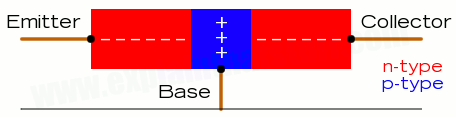
\includegraphics[width=0.5\textwidth]{figures/transistor2.png}
\caption{\label{fig:transistor2} A bipolar junction transistor, off-state.}
\end{figure}
\end{frame}

\begin{frame}{Introduction to transistors}
\begin{itemize}
\item How does a mixer use the transistor?
\item \alert{How does a transistor work?}
\item We will use this as an opportunity to learn how transistors may be used to form digital circuits.
\end{itemize}
\begin{figure}
\centering
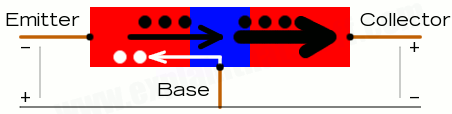
\includegraphics[width=0.5\textwidth]{figures/transistor3.png}
\caption{\label{fig:transistor3} A bipolar junction transistor, on-state.  Notice two things a) amplification and b) the switching effect.}
\end{figure}
\end{frame}

\begin{frame}{Introduction to transistors}
\begin{itemize}
\item How does a mixer use the transistor?
\item \alert{How does a transistor work?}
\item We will use this as an opportunity to learn how transistors may be used to form digital circuits.
\end{itemize}
\begin{figure}
\centering
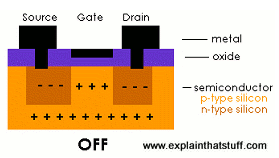
\includegraphics[width=0.4\textwidth]{figures/mosfet1.png}
\caption{\label{fig:mosfet1} A metal oxide field effect transistor, off-state.}
\end{figure}
\end{frame}

\begin{frame}{Introduction to transistors}
\begin{itemize}
\item How does a mixer use the transistor?
\item \alert{How does a transistor work?}
\item We will use this as an opportunity to learn how transistors may be used to form digital circuits.
\end{itemize}
\begin{figure}
\centering
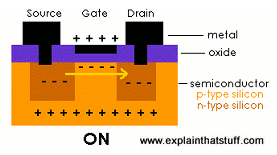
\includegraphics[width=0.4\textwidth]{figures/mosfet2.png}
\caption{\label{fig:mosfet2} A metal oxide field effect transistor, on-state.  The electric field created by the gate polarizes a channel between the source and drain, allowing current to flow.}
\end{figure}
\end{frame}

\section{The 2P3 Superheterodyne AM radio receiver}

\begin{frame}{The 2P3 Superheterodyne AM radio receiver}
\begin{figure}
\centering
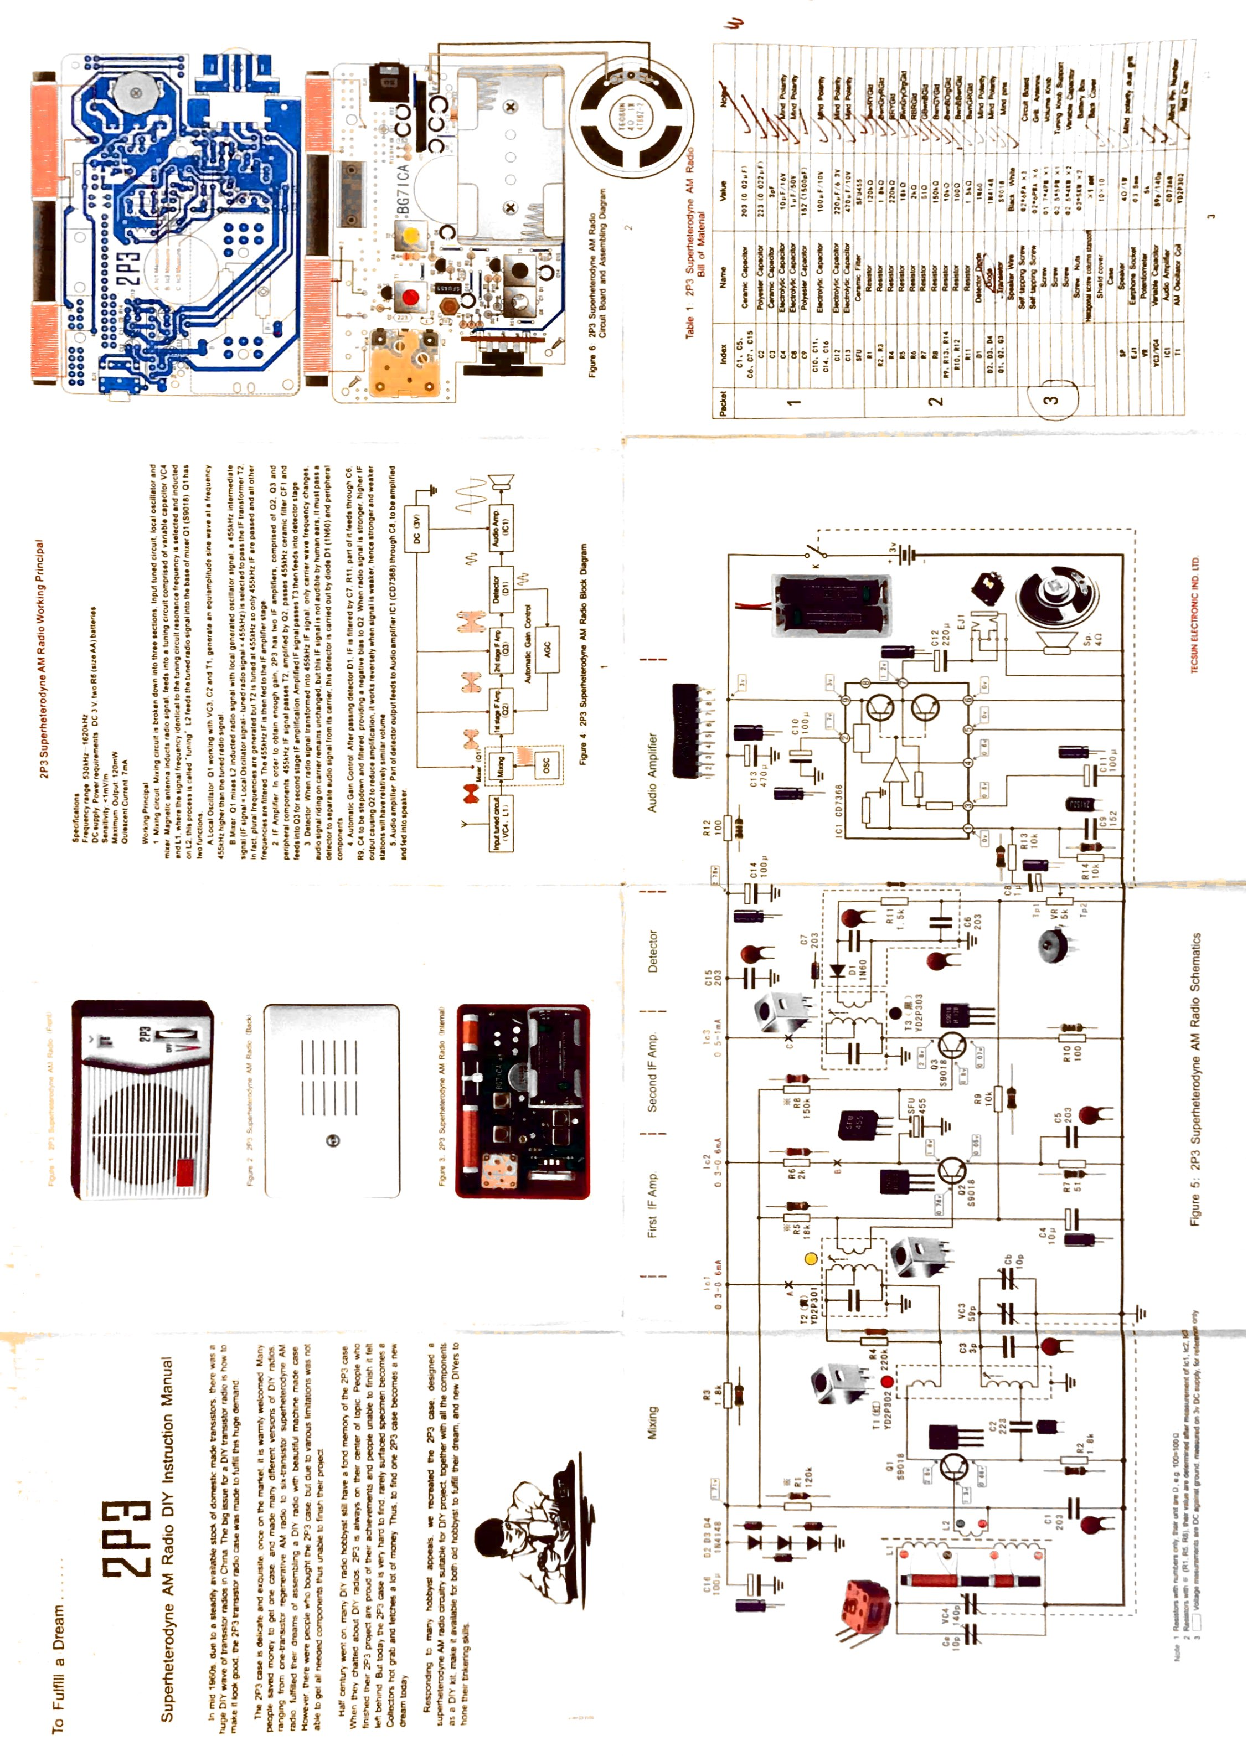
\includegraphics[width=0.55\textwidth,angle=270,trim=10.5cm 1.75cm 0cm 9cm,clip=true]{figures/2P3.pdf}
\caption{\label{fig:2P3} Where are the transistors in this AM transistor superhet?  What roles do they play in each case?}
\end{figure}
\end{frame}

\begin{frame}{The 2P3 Superheterodyne AM radio receiver}
\begin{figure}
\centering
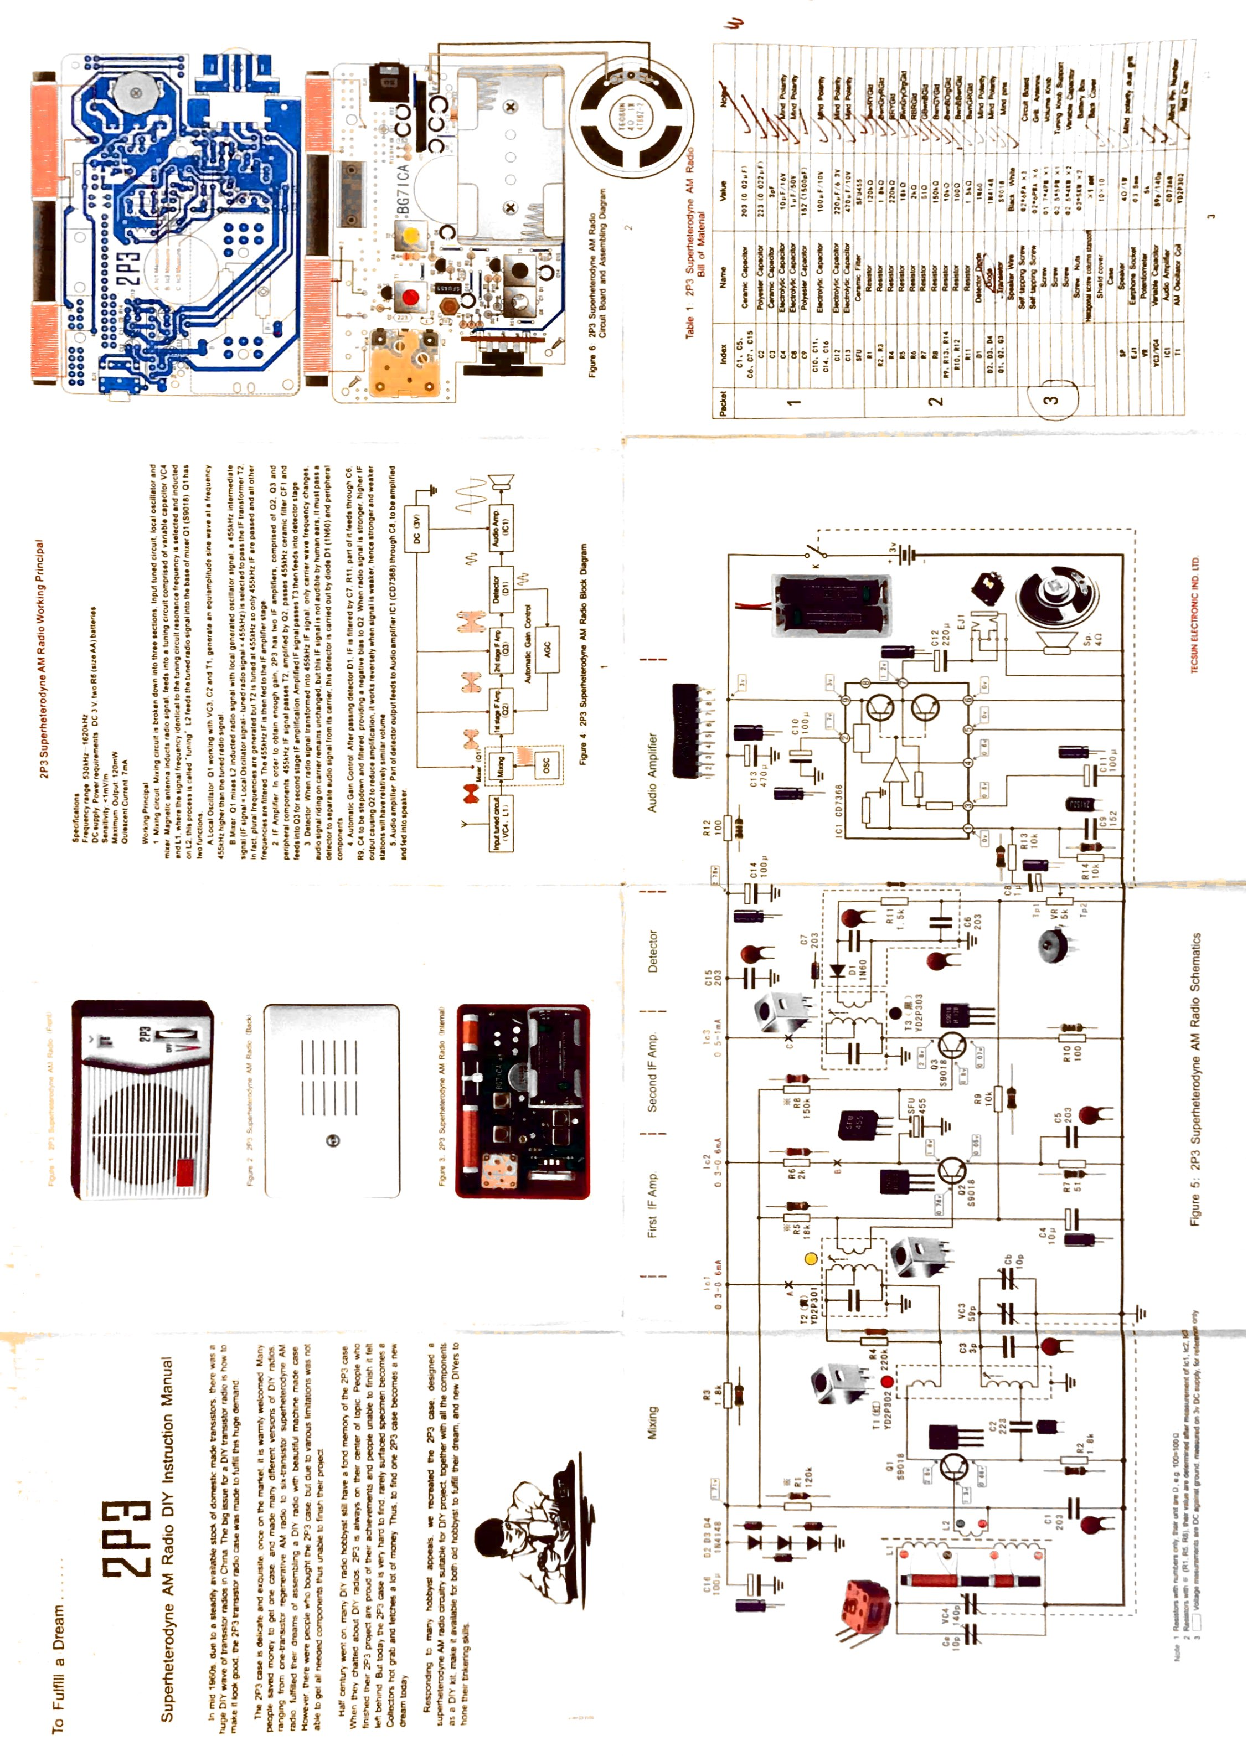
\includegraphics[width=0.6\textwidth,angle=270,trim=0cm 22.5cm 9cm 0cm,clip=true]{figures/2P3.pdf}
\caption{\label{fig:2P32} Through-hole style circuit board.}
\end{figure}
\end{frame}

\begin{frame}{The 2P3 Superheterodyne AM radio receiver}
\begin{figure}
\centering
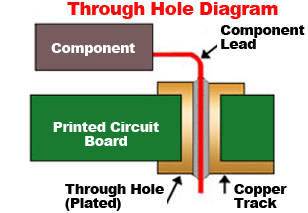
\includegraphics[width=0.65\textwidth]{figures/throughhole.png}
\caption{\label{fig:throughhole} Through-hole style circuit board.  By heating the copper (or other metal) track and the component lead, we may allow \textit{solder} to flow onto the heated areas, binding them together in a conductive fashion.}
\end{figure}
\end{frame}

\begin{frame}{The 2P3 Superheterodyne AM radio receiver}
\begin{figure}
\centering
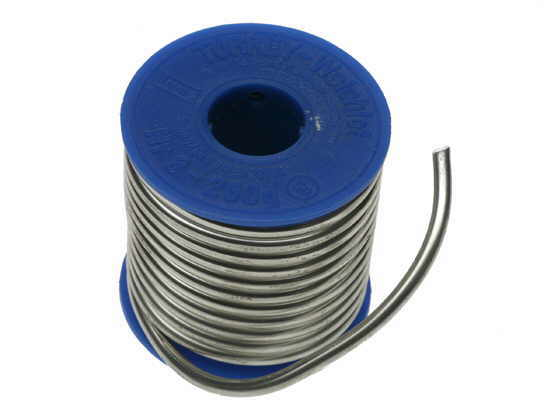
\includegraphics[width=0.3\textwidth,trim=0cm 0cm 2cm 0cm,clip=true]{figures/solder.png}
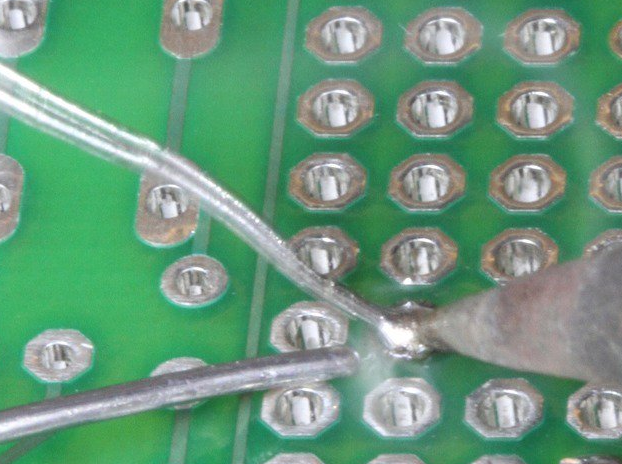
\includegraphics[width=0.4\textwidth]{figures/solder3.png}
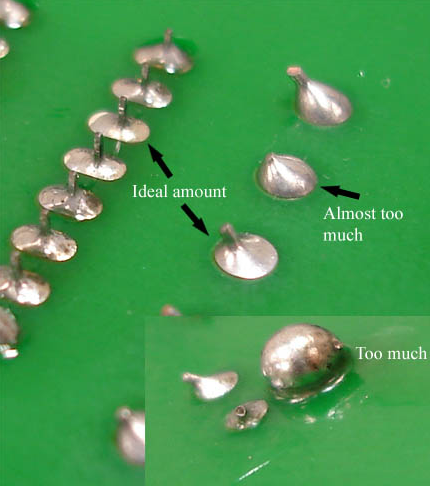
\includegraphics[width=0.3\textwidth]{figures/solder2.png}
\caption{\label{fig:soldering} (Left) Solder, used to bind components to board.  (Middle) Example of soldering iron causing solder to flow onto the heated hole. (Right) Exampls of correct and incorrect soldering.}
\end{figure}
\end{frame}

\begin{frame}{The 2P3 Superheterodyne AM radio receiver}
\begin{figure}
\centering
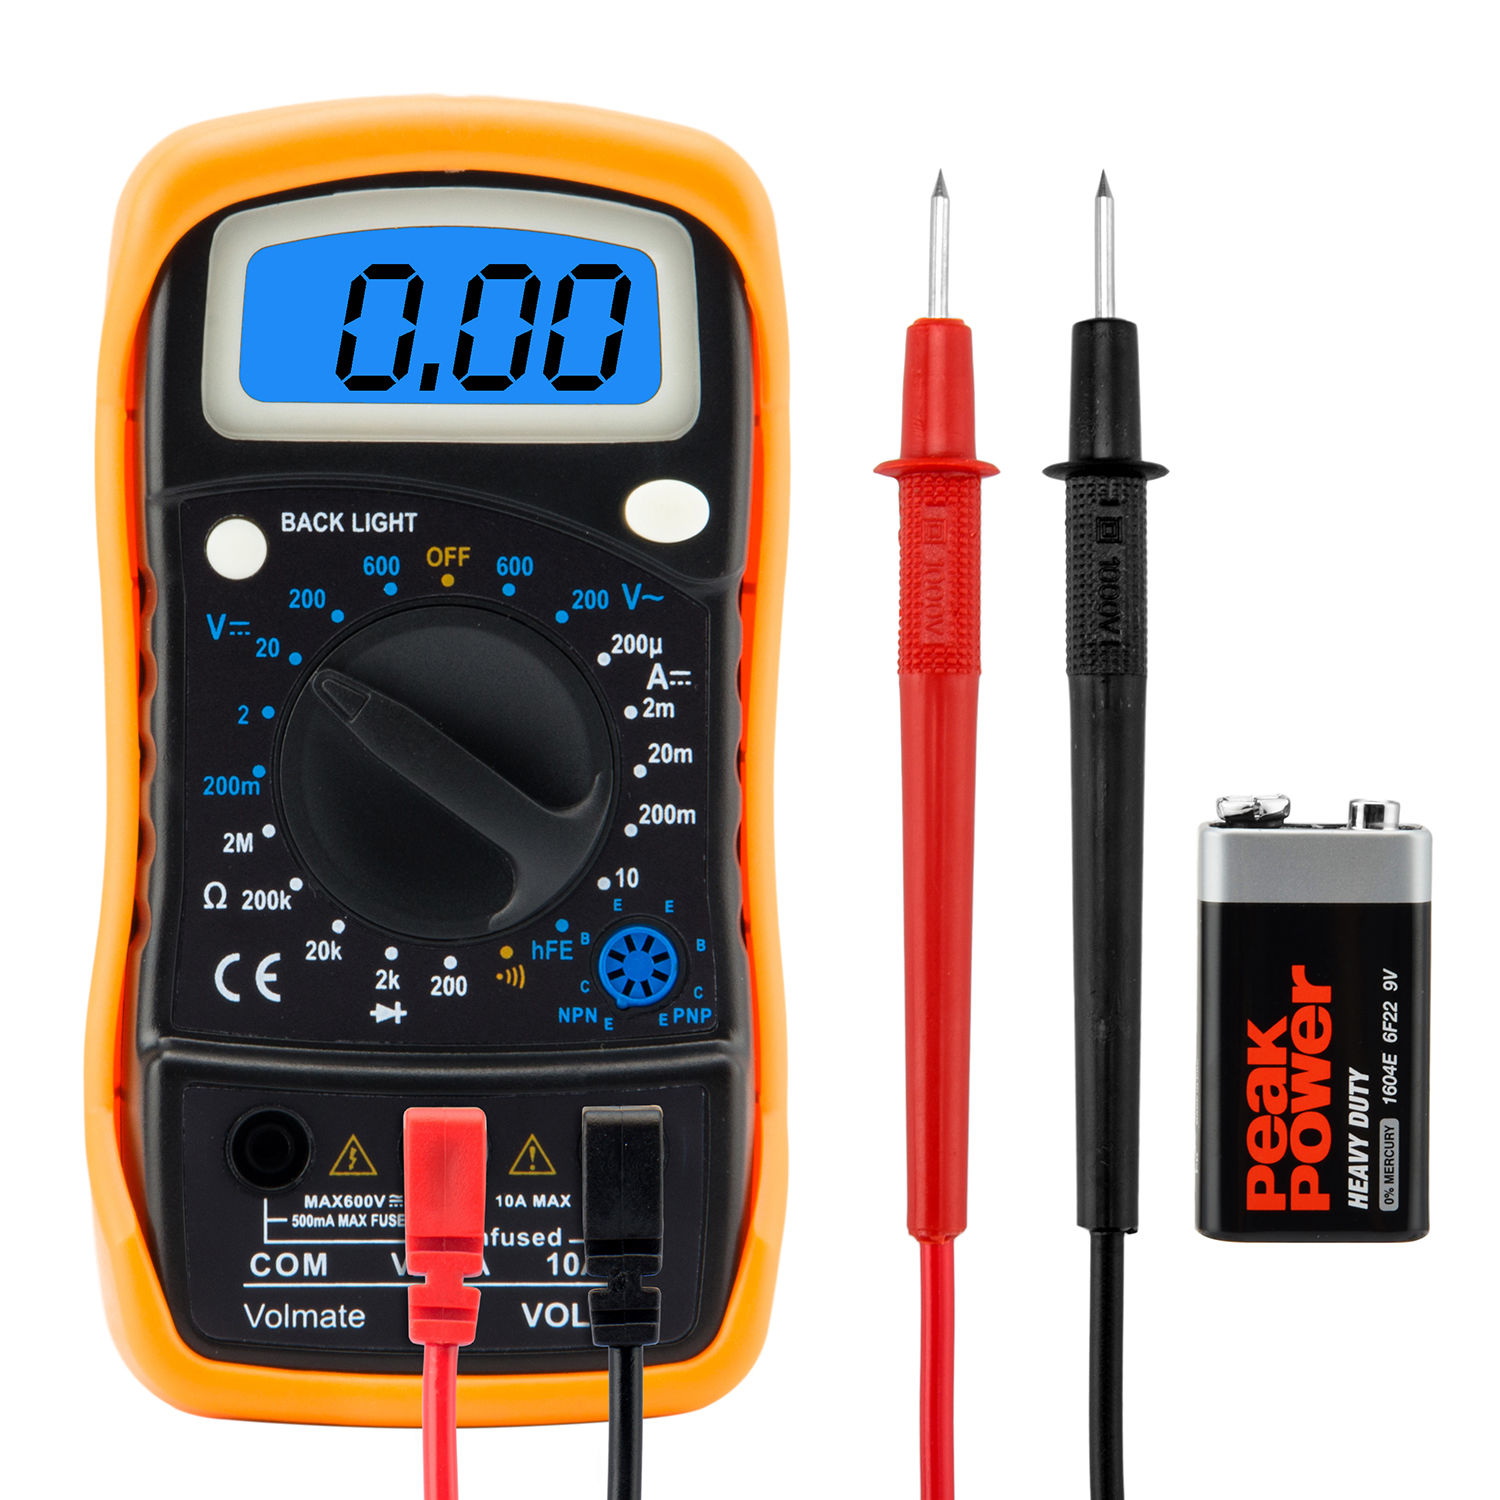
\includegraphics[width=0.5\textwidth]{figures/dvm.jpg}
\caption{\label{fig:dvm} The digital voltmeter (DVM) has three main functions: measuring voltage (voltmeter), measuring current (ammeter), and measuring conduction (the beep).}
\end{figure}
\end{frame}

\section{Build}

\section{Conclusion}

\begin{frame}{Unit 1.2 Summary - Build a radio from a pile of parts...go!}
\begin{enumerate}
\item Introduction to \textit{mixing} or \alert{heterodyning}
\begin{itemize}
\item The \textbf{transistor} plays a dual role
\item \textbf{Transistors} $\rightarrow$ forthcoming units on logic gates
\end{itemize}
\item The superheterodyne (superhet) radio receiver
\item Through-hole soldering 101
\item The DVM (digital voltmeter)
\item \textbf{Build.} $\rightarrow$ Bonus point for the first team
\end{enumerate}
\end{frame}

\end{document}
